\chapter{神经元、动作电位与突触}\label{ch:b2:neurons-synapses}

叩击膝盖骨下方的肌腱，小腿便会踢起，三十
毫秒之后。在这段时间内，大腿中感受到了牵张，
一个信号沿神经传送一米到达脊髓，越过一个连接，
进入第二个细胞，再沿原路返回一米，使一块肌肉
收缩——整个往返比眨眼还快。没有任何
\omterm{def:b2:cell-signalling:kinds}{激素}能做到这一点；这靠的是为传导而构造的细胞，以及
一种并非物质移动、而是电波的信号，电波沿膜不断再生。
本章讨论的正是这种细胞和这种信号：\omterm{def:b2:neurons-synapses:neuron}{神经元}在膜两侧维持的
电压、它所发出的冲动及冲动如何传播，以及
\omterm{def:b2:neurons-synapses:synapse}{突触}——在那里，电信号转变为化学信号，
再转变回电信号。

\section{神经元}

\begin{definition}[神经元、轴突、神经]\label{def:b2:neurons-synapses:neuron}
\index{神经元}\index{轴突}\index{树突}\index{髓鞘}\index{神经胶质}
\emph{神经元}是专司信号传递的细胞：一个细胞体
（\emph{胞体}）内含细胞核，分支状的\emph{树突}负责接收信号，
另有一根单独的\emph{轴突}——一条缆线，直径
从一微米到二十微米，长可达一米——
将其输出传送到其他细胞上的\emph{末端}。人脑约有
$10^{11}$ 个神经元，每个神经元约形成
一千个\omterm{def:b2:neurons-synapses:synapse}{突触}。神经元的数量远少于\emph{神经胶质}：星形胶质细胞
为神经元提供营养、缓冲其环境，小胶质细胞负责监视，以及
包裹轴突形成\emph{髓鞘}的细胞——其自身细胞膜绕行数十圈，
几乎不含细胞质，形成绝缘鞘，
约每隔一毫米即在\emph{郎飞结}处中断。
\emph{神经}是成千上万根轴突的束，包括感觉与运动两类，
在结缔组织中并行穿行。神经元在成体中一般不再分裂（少数例外），
与胞体断开的轴突即会死亡；神经元
是必须维持一生的细胞。
\end{definition}

\begin{omfigure}
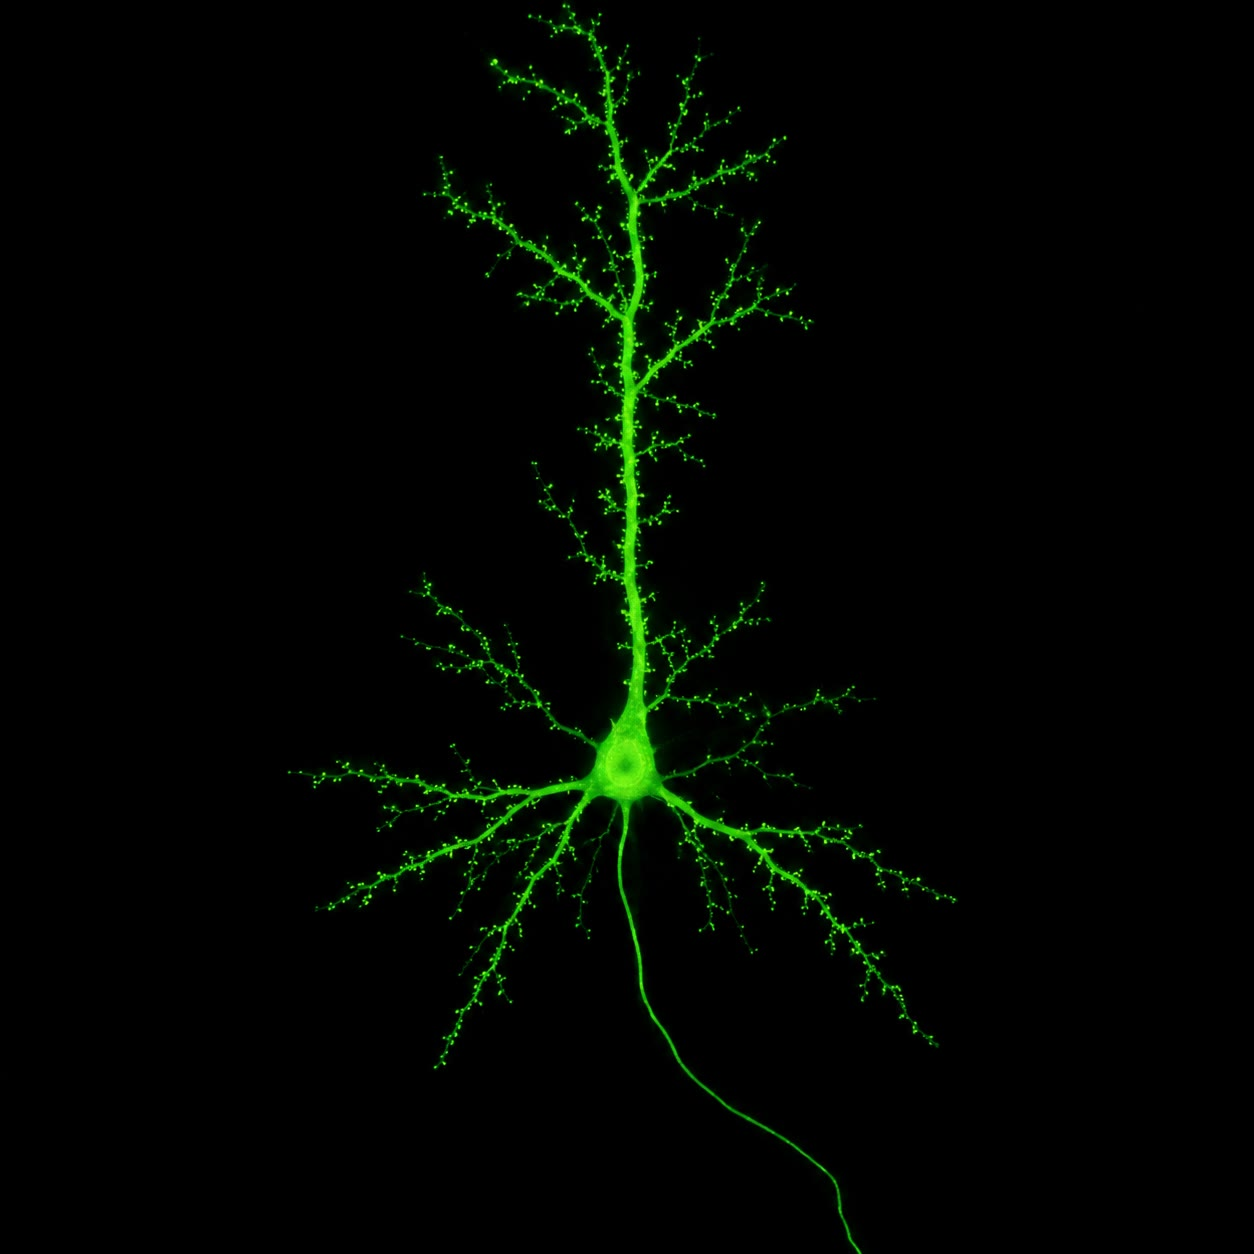
\includegraphics[width=0.4\linewidth]{images/book4/ai/b4-20-neuron-fluorescence.jpg}\hspace{0.05\linewidth}
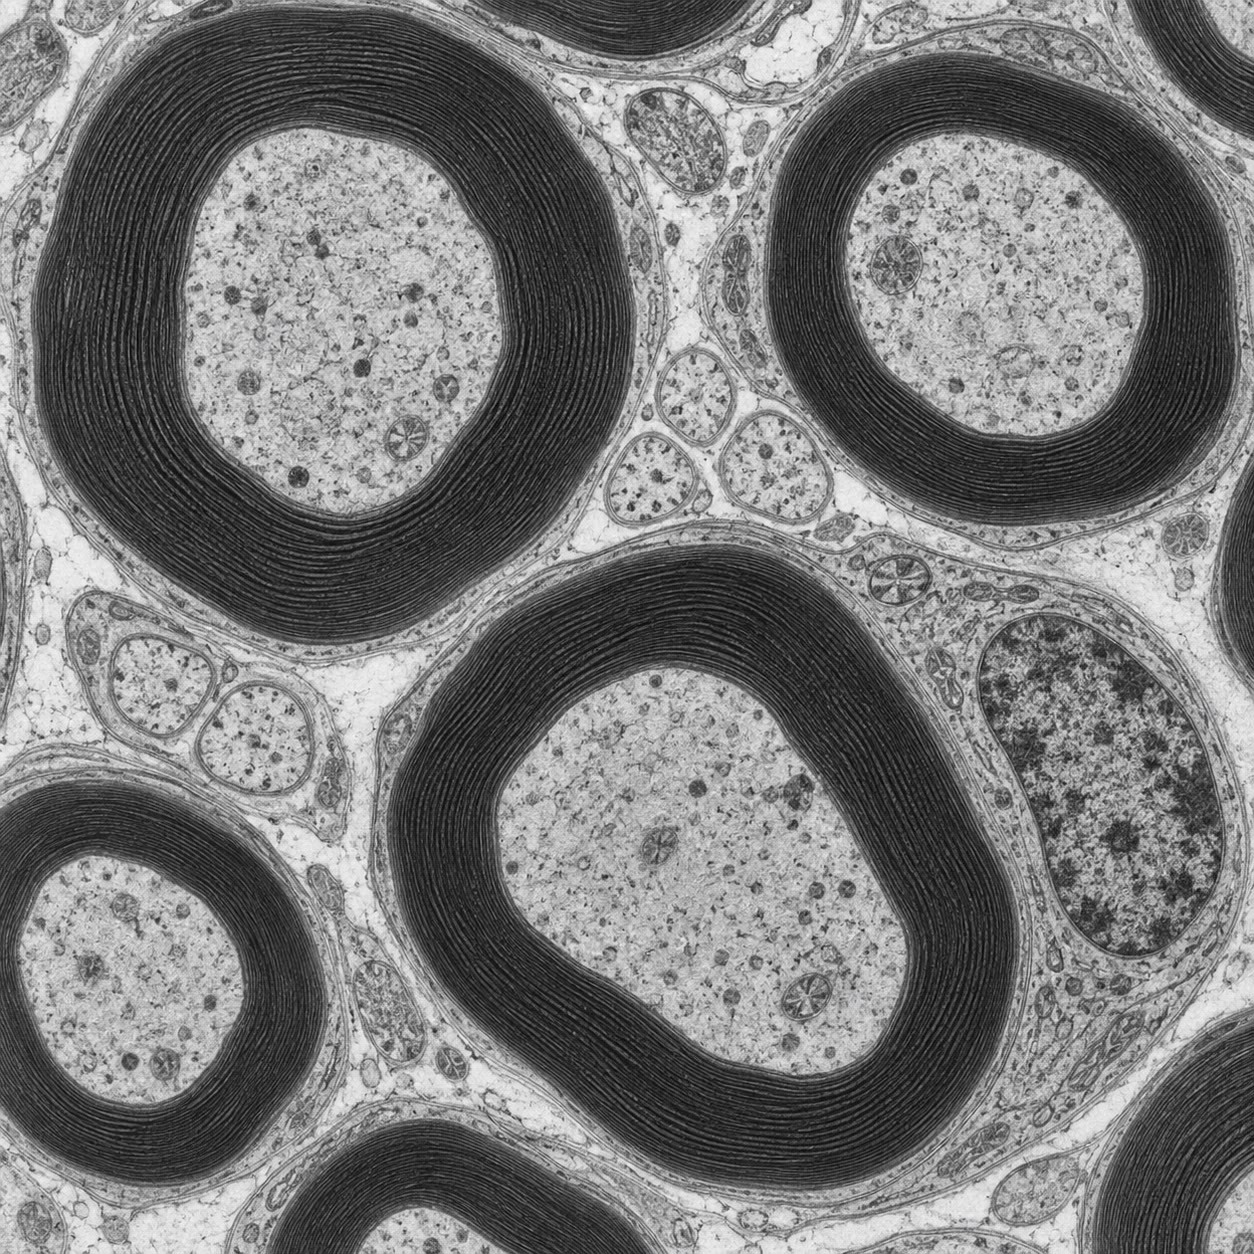
\includegraphics[width=0.4\linewidth]{images/book4/ai/b4-20-myelinated-axons-tem.jpg}

{\small 左：用染料充满的锥体\omterm{def:b2:neurons-synapses:neuron}{神经元}——细胞体、
带棘的\omterm{def:b2:neurons-synapses:neuron}{树突}（负责接收信号），以及细\omterm{def:b2:neurons-synapses:neuron}{轴突}从
基部发出。右：电子显微镜下的\omterm{def:b2:neurons-synapses:neuron}{轴突}横截面，
每根\omterm{def:b2:neurons-synapses:neuron}{轴突}外包深色螺旋状的\omterm{def:b2:neurons-synapses:neuron}{髓鞘}。}
\end{omfigure}

\section{静息电位}

\begin{theorem}[能斯特电位]\label{thm:b2:neurons-synapses:nernst}
\index{能斯特电位}\index{平衡电位}
对电荷为 $z$ 的某种离子可通透的膜，两侧
浓度分别为 $c_{\text{外}}$ 与 $c_{\text{内}}$，膜电位稳定在
\emph{\omterm{thm:b2:neurons-synapses:nernst}{平衡电位}}上，此时离子所受的电场力
与其扩散作用相平衡：
\[
E = \frac{RT}{zF}\ln\frac{c_{\text{外}}}{c_{\text{内}}} \approx \frac{\qty{61.5}{mV}}{z}\log_{10}\frac{c_{\text{外}}}{c_{\text{内}}} \quad (\qty{37}{\celsius}).
\]
\omterm{def:b2:neurons-synapses:neuron}{神经元}内钾离子为 \qty{140}{mmol/L}，细胞外为
\qty{5}{mmol/L}；钠离子在细胞内为 \qty{15}{mmol/L}，
细胞外为 \qty{145}{mmol/L}。这些梯度由
钠钾泵建立，代价是细胞三分之一的 ATP。
由此 $E_{\mathrm K} = 61.5\log_{10}(5/140) = \qty{-89}{mV}$，而
$E_{\mathrm{Na}} = 61.5\log_{10}(145/15) = \qty{+61}{mV}$：若膜
只允许钾通过，膜电位将稳定在
\qty{-89}{mV}；只允许钠通过则为 \qty{+61}{mV}。
\end{theorem}
\begin{proof}
平衡时，该离子的电化学势在膜两侧相同：
$RT\ln c_{\text{内}} + zFV_{\text{内}} = RT\ln
c_{\text{外}} + zFV_{\text{外}}$，故 $V_{\text{内}} -
V_{\text{外}} = (RT/zF)\ln(c_{\text{外}}/c_{\text{内}})$。在
温度 \qty{310}{K} 时，$RT/F = \qty{26.7}{mV}$，且 $\ln 10 \times 26.7 =
\qty{61.5}{mV}$。（该式在本科一年级分册中由玻尔兹曼
分布导出，此处重述。）
\end{proof}

\begin{theorem}[作为加权平均的静息电位]\label{thm:b2:neurons-synapses:chord}
\index{静息电位}\index{膜电导}
若膜同时传导几种离子，每种离子的电导为 $g_i$
（即离子通过的难易程度，由开放通道的数目决定），
则使电流相互抵消的稳态电位为
\[
V = \frac{\sum_i g_i E_i}{\sum_i g_i},
\]
各\omterm{thm:b2:neurons-synapses:nernst}{平衡电位}以电导为权重的加权平均。
静息时，\omterm{def:b2:neurons-synapses:neuron}{神经元}膜对钾的通透性约为对钠的二十倍，
故 $V \approx (20\times(-89) +
61)/21 = \qty{-82}{mV}$；计入氯离子与小的漏电流后，
\omterm{thm:b2:neurons-synapses:chord}{静息电位}为 \qty{-70}{mV}。膜之所以静息于
接近 $E_{\mathrm K}$ 处，是因为钾通道开放；任何
能打开钠通道的因素都会把膜电位拉向 $E_{\mathrm{Na}}$——这
正是神经信号传导的全部原理。
\end{theorem}
\begin{proof}
每种离子携带电流 $I_i = g_i(V - E_i)$（欧姆定律，驱动力
以该离子自身的\omterm{thm:b2:neurons-synapses:nernst}{平衡电位}为基准）。在某一
稳态电位下，总电流为零：$\sum_i g_i(V - E_i) =
0$，于是 $V\sum g_i = \sum g_iE_i$。（完整处理中，
通透性经由戈德曼–霍奇金–卡茨方程进入，
一级近似下给出相同的加权。）
\end{proof}

\section{动作电位}

\begin{proposition}[冲动]\label{prop:b2:neurons-synapses:ap}
\index{动作电位}\index{电压门控通道}\index{阈值}\index{不应期}
\omterm{def:b2:neurons-synapses:neuron}{轴突}膜上有\emph{电压门控钠通道}，静息时关闭，
去极化时开放。若刺激使膜电位由
\qty{-70}{mV} 上升，越过约 \qty{-55}{mV} 的\emph{阈值}，
足够多的钠通道开放，使流入的钠超过
钾漏电流所能抵消的量；电位继续上升，更多通道开放，
在不到一毫秒内膜电位即被迅速拉向
$E_{\mathrm{Na}}$——这是一种\emph{正反馈}，来势猛烈
且呈全或无的性质。峰值接近 \qty{+40}{mV}，原因在于钠通道
在开放后一毫秒之内即\emph{失活}，同时
较慢的\emph{电压门控钾通道}开放，
将电位拉回 $E_{\mathrm K}$ 附近，并超射至
\emph{后超极化}，之后钾通道才关闭。
\emph{\omterm{prop:b2:neurons-synapses:ap}{动作电位}}持续约一毫秒；此后再过一两毫秒，
失活的钠通道不能再次开放
（即\emph{\omterm{prop:b2:neurons-synapses:ap}{不应期}}），这将放电频率限制在
每秒数百次以内，并迫使冲动只能单向传播。
由于\omterm{prop:b2:neurons-synapses:ap}{动作电位}呈全或无，冲动的大小不携带信息，
\omterm{def:b2:neurons-synapses:neuron}{神经元}以其\emph{频率}编码强度。每次冲动约有
$10^{4}$ 个钠离子内流，同样数目的钾离子外流，
浓度变化可忽略，由
钠钾泵从容地恢复。
\end{proposition}
\begin{proof}[证据]
霍奇金与赫胥黎（1952 年）利用乌贼的巨大\omterm{def:b2:neurons-synapses:neuron}{轴突}（
粗约半毫米，可穿入一根细丝）和一台
反馈放大器，能将膜电位钳制在任意选定值
（即\emph{电压钳}），同时记录维持该电位所需的电流，
并将电流分离为较早的内向成分，
该成分在浴液中去除钠后消失；另有较晚的
外向成分由钾携带；测量了各电导在每一电压下
随时间如何升降；并用若干方程拟合每一成分，
由此算出\omterm{prop:b2:neurons-synapses:ap}{动作电位}的形状、
阈值、速度与\omterm{prop:b2:neurons-synapses:ap}{不应期}，全部仅由两种电导推出。
所有预测均得到证实。通道本身
直到二十五年后，才借助膜片钳逐个观察到。
河豚毒素（河豚体内的毒素）阻断钠通道，
从而取消冲动；四乙铵阻断钾通道，
并使\omterm{prop:b2:neurons-synapses:ap}{动作电位}延长。
\end{proof}

\begin{omfigure}
\begin{tikzpicture}
\begin{axis}[
  width=0.9\linewidth, height=6.4cm,
  axis x line=bottom, axis y line=left,
  xmin=0, xmax=4, ymin=-100, ymax=60,
  xlabel={时间（ms）}, ylabel={膜电位（mV）},
  xlabel style={font=\small, at={(axis description cs:0.5,-0.1)}, anchor=north},
  ylabel style={font=\small},
  tick label style={font=\small}, xtick={0,1,2,3,4}, ytick={-90,-70,-55,0,40},
  legend style={font=\scriptsize, at={(0.97,0.95)}, anchor=north east, draw=none},
  clip=false,
]
\addplot[very thick, omDef] coordinates {(0,-70) (0.4,-70) (0.5,-64) (0.6,-55) (0.7,-30) (0.8,10) (0.9,35) (1.0,40) (1.1,30) (1.2,10) (1.35,-20) (1.5,-50) (1.7,-75) (1.9,-85) (2.2,-82) (2.6,-76) (3.2,-71) (4,-70)};
\addlegendentry{膜电位}
\addplot[thick, omThm, dashed] coordinates {(0,0) (0.5,0) (0.6,5) (0.7,20) (0.8,35) (0.9,30) (1.0,20) (1.1,8) (1.2,3) (1.4,0) (4,0)};
\addlegendentry{$g_{\mathrm{Na}}$（相对值）}
\addplot[thick, omProp, dashed] coordinates {(0,0) (0.6,0) (0.8,2) (1.0,8) (1.2,16) (1.4,20) (1.7,17) (2.0,10) (2.4,4) (3.0,1) (4,0)};
\addlegendentry{$g_{\mathrm K}$（相对值）}
\draw[dashed, gray] (axis cs:0,-55) -- (axis cs:4,-55); \node[font=\scriptsize, anchor=south east] at (axis cs:4,-55) {阈值};
\draw[dashed, gray] (axis cs:0,-89) -- (axis cs:4,-89); \node[font=\scriptsize, anchor=south east] at (axis cs:3.7,-89) {$E_{\mathrm K}$};
\draw[<->, gray] (axis cs:1.0,50) -- (axis cs:2.5,50); \node[font=\scriptsize, anchor=south, gray] at (axis cs:1.75,50) {不应期};
\end{axis}
\end{tikzpicture}

{\small 一个\omterm{prop:b2:neurons-synapses:ap}{动作电位}。越过阈值后，钠电导
（红色）急剧上升，并将电位推向
$E_{\mathrm{Na}}$；随后钾电导
（橙色）上升，使其失活，并使膜电位回落向 $E_{\mathrm K}$，
并出现超射。阈值线以下，不发生任何变化。}
\end{omfigure}

\section{传导}

\begin{theorem}[电缆与长度常数]\label{thm:b2:neurons-synapses:cable}
\index{长度常数}\index{电缆方程}\index{传导速度}
\omterm{def:b2:neurons-synapses:neuron}{轴突}是一根有漏电的电缆：在某点注入的电流沿
细胞质流动（每单位长度的电阻为 $r_i$），并
经膜向外漏出（电阻为 $r_m$ 与单位长度之积）。稳定
去极化 $V_0$ 作用于 $x = 0$ 处，沿\omterm{def:b2:neurons-synapses:neuron}{轴突}按
\[
V(x) = V_0\,e^{-x/\lambda}, \qquad \lambda = \sqrt{\frac{r_m}{r_i}} = \sqrt{\frac{R_m\,d}{4R_i}},
\]
衰减，其中 $d$ 为直径，$R_m$、$R_i$ 分别为膜和
细胞质的比电阻。\emph{\omterm{thm:b2:neurons-synapses:cable}{长度常数}}
$\lambda$ 是被动信号衰减至
三分之一时所经过的距离：约为 \qty{0.5}{mm}（对于直径为 \qty{1}{\micro m} 的\omterm{def:b2:neurons-synapses:neuron}{轴突}），
并随直径的平方根增大。\omterm{prop:b2:neurons-synapses:ap}{动作电位}之所以能传播，是因为
其前端的去极化被动地向前扩散
约 $\lambda$ 的距离，使下一段膜达到
阈值，从而使其以全幅度再生；波前到达得越远，
波速越快，因此\omterm{thm:b2:neurons-synapses:cable}{传导速度}也
大致随 $\sqrt{d}$ 增大——从细的
无髓纤维中的 \qty{1}{m/s}，到乌贼巨\omterm{def:b2:neurons-synapses:neuron}{轴突}中的 \qty{20}{m/s}。
\end{theorem}
\begin{proof}
设 $i(x)$ 为轴向电流，$V(x)$ 为膜
去极化量。沿轴浆应用欧姆定律得 $\mathrm{d}V/
\mathrm{d}x = -r_i\,i$；由电荷守恒（计入经膜的漏电），
得 $\mathrm{d}i/\mathrm{d}x = -V/r_m$。联立两式，
$\mathrm{d}^{2}V/\mathrm{d}x^{2} = V/(r_m r_i)$，其衰减解
为 $V_0 e^{-x/\lambda}$，且 $\lambda^{2} = r_m/r_i$。对圆柱体而言，
$r_m = R_m/(\pi d)$，$r_i = 4R_i/(\pi d^{2})$，故
$\lambda^{2} = R_m d/4R_i$。取 $R_m = \qty{1}{\ohm.m^2}$，$R_i =
\qty{1}{\ohm.m}$，$d = \qty{1}{\micro m}$，则 $\lambda = \sqrt{10^{-6}
/4} = \qty{0.5}{mm}$。
\end{proof}

\begin{proposition}[髓鞘与跳跃式传导]\label{prop:b2:neurons-synapses:myelin}
\index{跳跃式传导}\index{郎飞结}
\omterm{def:b2:neurons-synapses:neuron}{髓鞘}使 $r_m$ 增大为原来的膜转角数倍，同时
使膜电容减小为原来的同一倍数，从而在\omterm{def:b2:neurons-synapses:neuron}{髓鞘}之下
几乎没有电流漏出，改变电位所需的电荷很少：
去极化可沿约一毫米长的\omterm{def:b2:neurons-synapses:neuron}{髓鞘}节间被动扩散，
损失很小，\omterm{prop:b2:neurons-synapses:ap}{动作电位}仅在
郎飞结处再生，而这里正是钠通道集中的位置。
冲动因此从一个结\emph{跃过}到下一个结
（\emph{\omterm{prop:b2:neurons-synapses:myelin}{跳跃式传导}}），速度达 \qty{100}{m/s}，
在直径为 \qty{20}{\micro m} 的纤维中——无髓\omterm{def:b2:neurons-synapses:neuron}{轴突}要达到这一速度，
需要粗到几厘米才行——而且代谢代价只是
其一小部分，因为钠只在结处内流。\omterm{def:b2:neurons-synapses:neuron}{髓鞘}是
脊椎动物的一项创新，使小型身体中也能拥有庞大而快速的神经系统；
在多发性硬化症中，\omterm{def:b2:neurons-synapses:neuron}{髓鞘}逐片
被破坏，\omterm{thm:b2:neurons-synapses:cable}{长度常数}随之崩溃，冲动也就
无法传导。
\end{proposition}

\begin{omfigure}
\begin{tikzpicture}[every node/.style={font=\scriptsize}, >=stealth]
  % unmyelinated
  \begin{scope}
    \draw[thick, fill=omDef!10] (0,0) rectangle (11,0.5);
    \foreach \x in {0.5,1.0,...,10.5} \draw[omThm, ->] (\x,0.25) -- (\x,0.9);
    \node[anchor=east] at (-0.2,0.25) {无髓};
    \node[anchor=west] at (11.2,0.25) {\qty{1}{m/s}};
    \node[above] at (5.5,1.0) {冲动在每一点都被再生};
  \end{scope}
  % myelinated
  \begin{scope}[yshift=-2.4cm]
    \draw[thick, fill=omDef!10] (0,0) rectangle (11,0.5);
    \foreach \x in {0.3,2.5,4.7,6.9,9.1} \fill[omExo!60] (\x,-0.15) rectangle (\x+1.9,0.65);
    \foreach \x in {2.35,4.55,6.75,8.95} \draw[omThm, ->] (\x,0.25) -- (\x,0.9);
    \foreach \x in {2.35,4.55,6.75} \draw[->, thick, omThm, dashed] (\x+0.1,1.1) .. controls (\x+1.1,1.6) .. (\x+2.1,1.1);
    \node[anchor=east] at (-0.2,0.25) {有髓};
    \node[anchor=west] at (11.2,0.25) {\qty{100}{m/s}};
    \node[below] at (1.25,-0.2) {髓鞘节间};
    \node[below] at (4.55,-0.2) {郎飞结};
    \node[above] at (5.5,1.6) {仅在郎飞结处再生：跳跃式};
  \end{scope}
\end{tikzpicture}

{\small 有髓与无髓\omterm{def:b2:neurons-synapses:neuron}{轴突}中的传导。在裸露的\omterm{def:b2:neurons-synapses:neuron}{轴突}中，
冲动沿整条\omterm{def:b2:neurons-synapses:neuron}{轴突}不断再生；有\omterm{def:b2:neurons-synapses:neuron}{髓鞘}时，信号沿每个\omterm{def:b2:neurons-synapses:neuron}{髓鞘}节间被动传播，
仅在郎飞结处再生，
冲动的\omterm{thm:b2:neurons-synapses:cable}{传导速度}快约一百倍。}
\end{omfigure}

\section{突触}

\begin{definition}[化学突触与电突触]\label{def:b2:neurons-synapses:synapse}
\index{突触}\index{神经递质}\index{突触后电位}
在\emph{突触}处，\omterm{def:b2:neurons-synapses:neuron}{神经元}的末梢与一个靶细胞相接，
靶细胞可以是另一个\omterm{def:b2:neurons-synapses:neuron}{神经元}、\omterm{def:b2:cell-differentiation:myogenesis}{肌纤维}或腺细胞。在\emph{电突触}中，
缝隙连接将两个细胞相连，电流直接通过，
速度快、双向传递、无放大，
适用于对速度与同步性要求高的场合（逃避反射、\omterm{def:b2:heart:anatomy}{心脏}）。在\emph{化学突触}中，
两个细胞之间隔着宽\qty{20}{nm}的间隙，信号由
分子传递。到达末梢的\omterm{prop:b2:neurons-synapses:ap}{动作电位}
打开电压门控钙通道；钙离子内流，
在不到一毫秒的时间内，使含\emph{神经递质}的囊泡
与膜融合，并将递质释放到间隙中；
递质在微秒量级内扩散越过间隙，并与
突触后膜上的受体结合——受体可以是其打开的离子通道
（\emph{离子型}，速度快），或为\omterm{prop:b2:cell-signalling:gpcr}{G蛋白偶联受体}
（\emph{代谢型}，速度较慢，见\cref{ch:b2:cell-signalling}）；
所产生的电流使突触后电位改变数毫伏，
向上的为（\emph{兴奋性突触后电位}，通过钠通道内流），
或向下的为（\emph{抑制性}突触后电位，通过氯离子或钾离子的通道）；
递质在数毫秒内
被酶分解或被转运体回收。
延迟约为半毫秒；这一代价换来了单向传递、
放大、抑制与可塑性——
神经系统在单纯传导之外所需要的一切。
\end{definition}

\begin{omfigure}
\begin{tikzpicture}[every node/.style={font=\scriptsize}, >=stealth]
  % presynaptic terminal
  \draw[thick, fill=omDef!10] (0,0) .. controls (0,2.6) and (3.6,2.6) .. (3.6,0.2) -- (3.6,-0.2) .. controls (3.6,-2.6) and (0,-2.6) .. (0,0);
  \draw[very thick, omDef] (-2.2,0) -- (0.1,0); \node[omDef, above] at (-1.1,0.05) {轴突};
  \foreach \p in {(2.0,1.0),(2.6,0.5),(2.7,-0.4),(2.1,-1.0),(1.6,0.2)} \draw[thick, fill=omProp!40] \p circle (0.25);
  \draw[thick, fill=omProp!40] (3.3,0.1) arc (90:-90:0.25) -- cycle;
  \foreach \p in {(3.75,0.2),(3.85,-0.1),(3.7,-0.35),(3.9,0.4)} \fill[omProp] \p circle (0.05);
  \fill[omThm] (3.45,1.3) circle (0.06); \node[omThm, anchor=east] at (3.35,1.45) {Ca$^{2+}$内流};
  \draw[->, omThm] (3.9,1.5) -- (3.55,1.35);
  % cleft
  \node[align=center, anchor=north] at (3.85,-2.75) {间隙 \\\qty{20}{nm}};
  \draw[gray] (3.85,-2.7) -- (3.85,-1.2);
  % postsynaptic
  \draw[thick, fill=omExo!15] (4.1,-2.6) rectangle (8.2,2.6);
  \foreach \y in {0.9,0.3,-0.3,-0.9} \draw[thick, fill=omDef!40] (4.05,\y-0.15) rectangle (4.45,\y+0.15);
  \node[anchor=west, align=left] at (4.6,0.3) {受体：通道 \\打开，离子流入，\\突触后 \\电位};
  \node[anchor=west, align=left] at (4.6,-1.7) {递质被移除 \\由酶或 \\转运体承担};
  \node[anchor=west] at (4.6,2.2) {突触后细胞};
  % labels
  \node[align=center, anchor=north] at (1.8,-2.75) {含递质的 \\囊泡};
  \node[anchor=south] at (1.8,2.75) {突触前末梢};
\end{tikzpicture}

{\small 化学\omterm{def:b2:neurons-synapses:synapse}{突触}。冲动使钙离子内流，囊泡
融合并将递质释放到间隙中，\omterm{def:b2:neurons-synapses:synapse}{突触}后膜的受体
随即打开通道，递质在
数毫秒内被清除。}
\end{omfigure}

\begin{theorem}[量子式释放]\label{thm:b2:neurons-synapses:quantal}
\index{量子式释放}\index{微小电位}
递质以“包”的形式释放，每一包称为\emph{量子}，
即一个囊泡，一次冲动所释放的量子数 $k$ 是
随机变量。若末梢有 $n$ 个释放位点，每个位点
以概率 $p$ 释放，且 $p$ 很小，$k$ 近似服从
均值为 $m = np$ 的泊松分布：
\[
P(k) = \frac{m^{k}e^{-m}}{k!}, \qquad P(0) = e^{-m}, \qquad
m = \ln\frac{\text{试验次数}}{\text{失效次数}}.
\]
因此，平均量子含量 $m$ 可由释放为零的
冲动所占比例读出，并可与
平均反应除以单个量子的大小相互核对。在
\omterm{prop:b2:neurons-synapses:integration}{神经肌肉接头}处，$m$ 为数百，
传递从不失效；在中枢\omterm{def:b2:neurons-synapses:synapse}{突触}处，常接近一，\omterm{def:b2:neurons-synapses:synapse}{突触}
只在一部分冲动上传递。
\end{theorem}
\begin{proof}
设有 $n$ 个独立位点，每个以概率 $p$ 释放，则 $k$
服从二项分布；当 $n$ 大、$p$ 小且 $np = m$ 固定时，
二项分布趋于泊松分布（见数学系列本科二年级分册）。
由 $P(0) = e^{-m}$，失效次数给出 $m$。卡茨的检验是
同一 $m$ 代入泊松公式，即可预测观测到的
一个、两个、三个量子反应所占的比例。
\end{proof}
\begin{proof}[证据]
法特与卡茨（1952）在静息的蛙\omterm{def:b2:cell-differentiation:myogenesis}{肌纤维}上记录到
约为\qty{0.5}{mV}的微小自发去极化，
大小相同，于随机时间间隔出现，
即\emph{微小终板电位}，每一个都是一个囊泡的效应。降低浴液中的钙离子浓度后，
神经刺激引起的反应下降，直至
在 0、1、2 或 3 倍\omterm{thm:b2:neurons-synapses:quantal}{微小电位}的大小之间波动；
各倍数出现的频率服从泊松定律，
所用的 $m$ 由失效次数算得。德尔卡斯蒂略与卡茨由此证明
释放是量子式的，钙离子控制的是释放概率，
而非量子的大小；电子显微镜
显示了作为量子的囊泡。
\end{proof}

\begin{proposition}[整合：神经元作为决策者]\label{prop:b2:neurons-synapses:integration}
\index{总和}\index{轴突起始段}\index{神经肌肉接头}
中枢\omterm{def:b2:neurons-synapses:neuron}{神经元}在其\omterm{def:b2:neurons-synapses:neuron}{树突}和胞体上接受数千个兴奋性与
抑制性\omterm{def:b2:neurons-synapses:synapse}{突触}的输入。每个\omterm{def:b2:neurons-synapses:synapse}{突触后电位}都很小，
并被动衰减，空间上以线缆的\omterm{thm:b2:neurons-synapses:cable}{长度常数}为尺度，
时间上以膜的时间常数（数毫秒）为尺度；
它们相加——同时到达的输入发生\emph{空间\omterm{prop:b2:neurons-synapses:integration}{总和}}，
快速相继到达的输入发生\emph{时间\omterm{prop:b2:neurons-synapses:integration}{总和}}——
\omterm{prop:b2:neurons-synapses:integration}{总和}值在\emph{\omterm{prop:b2:neurons-synapses:integration}{轴突起始段}}处被读取，该处钠通道最密集，
阈值最低。若\omterm{prop:b2:neurons-synapses:integration}{总和}超过阈值，
\omterm{def:b2:neurons-synapses:neuron}{轴突}便发放冲动，发放频率随超出量的增大而升高；
抑制性输入起减法作用，靠近起始段的抑制性\omterm{def:b2:neurons-synapses:synapse}{突触}
可以否决远处的兴奋性\omterm{def:b2:neurons-synapses:synapse}{突触}的作用。\omterm{prop:b2:neurons-synapses:integration}{神经肌肉接头}是
体现这一规律的例外：一个运动末梢释放数百个
乙酰胆碱量子，作用于兼作通道的受体上，
产生终板电位，
\qty{50}{mV}，远高于阈值——运动神经中的每一次冲动
都会产生一次肌肉\omterm{prop:b2:neurons-synapses:ap}{动作电位}，
（见\cref{ch:b2:muscle-movement}）。箭毒阻断受体，
导致麻痹；神经毒气阻断清除
乙酰胆碱的酶，则由相反的过量引起麻痹。
\end{proposition}

\begin{example}[神经递质与药物]\label{ex:b2:neurons-synapses:transmitters}
乙酰胆碱见于\omterm{prop:b2:neurons-synapses:integration}{神经肌肉接头}及\omterm{def:b2:blood-pressure:baroreflex}{自主神经系统}；
谷氨酸是脑内主要的兴奋性\omterm{def:b2:neurons-synapses:synapse}{神经递质}，
GABA 是主要的抑制性\omterm{def:b2:neurons-synapses:synapse}{神经递质}；单胺类包括去甲肾上腺素、
多巴胺和血清素，它们调节由几
千个细胞组成的整个回路；此外还有数十种肽。几乎所有作用于精神的
药物都作用于\omterm{def:b2:neurons-synapses:synapse}{突触}：苯二氮卓类增强 GABA 的
通道，抗抑郁药阻断血清素转运体，可卡因
阻断多巴胺转运体，阿片类药物模拟一种肽，尼古丁
在一种受体上模拟乙酰胆碱，阿托品则在另一种受体上阻断它，
肉毒毒素切断使囊泡融合的蛋白质。
\omterm{def:b2:neurons-synapses:synapse}{突触}是\cref{ch:b2:cell-signalling}中的化学与
本章的电学相遇之处，也是神经系统学习之处：
常用的\omterm{def:b2:neurons-synapses:synapse}{突触}会被增强，这种增强（
见本科三年级分册）即是记忆。
\end{example}

\section{练习}

\begin{exercise}[$\star$]\label{exo:b2:neurons-synapses:1}
说出\omterm{def:b2:neurons-synapses:neuron}{神经元}各组成部分及其功能，并说明
\omterm{def:b2:neurons-synapses:neuron}{髓鞘}由什么构成以及它的作用。
\end{exercise}

\begin{exercise}[$\star$]\label{exo:b2:neurons-synapses:2}
描述\omterm{prop:b2:neurons-synapses:ap}{动作电位}的各个时期，以及
各时期的通道事件。为何\omterm{prop:b2:neurons-synapses:ap}{动作电位}是“全或无”的，为何它不会向后
传导？
\end{exercise}

\begin{exercise}[$\star$]\label{exo:b2:neurons-synapses:3}
列出化学\omterm{def:b2:neurons-synapses:synapse}{突触}中从冲动到达至\omterm{def:b2:neurons-synapses:synapse}{神经递质}被清除的
全部传递步骤。
\end{exercise}

\begin{exercise}[$\star$]\label{exo:b2:neurons-synapses:4}
比较电\omterm{def:b2:neurons-synapses:synapse}{突触}与化学\omterm{def:b2:neurons-synapses:synapse}{突触}在速度、方向、
放大作用及能否产生抑制等方面的异同。
\end{exercise}

\begin{exercise}[$\star\star$]\label{exo:b2:neurons-synapses:5}
计算下列离子在 \qty{37}{\celsius} 时的\omterm{thm:b2:neurons-synapses:nernst}{能斯特电位}：钾
（胞内 140，胞外 5）、钠（胞内 15，胞外 145）、氯（胞内 10，胞外 110）
和钙（胞内 \qty{1e-4}{}，胞外 2，单位 \unit{mmol/L}）。
当膜电位为 \qty{-70}{mV} 时，各离子向何方向流动？
\end{exercise}

\begin{exercise}[$\star\star$]\label{exo:b2:neurons-synapses:6}
已知 $E_{\mathrm K} = \qty{-89}{mV}$ 和 $E_{\mathrm{Na}} =
\qty{+61}{mV}$，计算膜电位，当 $g_{\mathrm K} :
g_{\mathrm{Na}} = 20 : 1$（静息）、$1 : 20$（\omterm{prop:b2:neurons-synapses:ap}{动作电位}峰值）
以及 $50 : 1$（后超极化）。并说明每种状态。
\end{exercise}

\begin{exercise}[$\star\star$]\label{exo:b2:neurons-synapses:7}
无髓\omterm{def:b2:neurons-synapses:neuron}{轴突}中\omterm{thm:b2:neurons-synapses:cable}{传导速度}与 $\sqrt d$ 成正比，已知直径为
\qty{1}{\micro m} 时速度为 \qty{1}{m/s}。计算直径为
\qty{0.5}{mm} 的枪乌贼\omterm{def:b2:neurons-synapses:neuron}{轴突}的速度。一根直径为 \qty{20}{\micro m} 的有髓纤维
以 \qty{100}{m/s} 传导，无髓\omterm{def:b2:neurons-synapses:neuron}{轴突}须多粗才能与之相匹配？
冲动从脊髓传到脚趾（\qty{1}{m}）在
两种纤维中各需多长时间？
\end{exercise}

\begin{exercise}[$\star\star$]\label{exo:b2:neurons-synapses:8}
在低钙条件下对\omterm{def:b2:neurons-synapses:synapse}{突触}进行 200 次刺激，其中 74 次
未产生反应。计算平均量子含量及
预测的产生一、二、三个量子反应的比例。单个量子
的幅度为 \qty{0.5}{mV}，预期的平均反应为多大？
\end{exercise}

\begin{exercise}[$\star\star$]\label{exo:b2:neurons-synapses:9}
\omterm{def:b2:neurons-synapses:neuron}{神经元}的\omterm{prop:b2:neurons-synapses:ap}{不应期}为 \qty{2}{ms}。其最高
放电频率是多少？一感觉\omterm{def:b2:neurons-synapses:neuron}{神经元}轻触时每秒发放 20 次
冲动，用力触压时发放 200 次。所编码的是何种信息，以何种方式编码？
\end{exercise}

\begin{exercise}[$\star\star\star$]\label{exo:b2:neurons-synapses:10}
计算 $R_m = \qty{1}{\ohm.m^2}$，$R_i =
\qty{1}{\ohm.m}$ 时的\omterm{thm:b2:neurons-synapses:cable}{长度常数}，直径分别为 1、10 和 \qty{500}{\micro m}。\omterm{def:b2:neurons-synapses:neuron}{髓鞘}
使 $R_m$ 乘以 200：对 \qty{10}{\micro m} 的情形重新计算。说明
为何长 \qty{1}{mm} 的节间能正常工作，而
脱\omterm{def:b2:neurons-synapses:neuron}{髓鞘}的 \qty{3}{mm} 长段会阻断冲动。
\end{exercise}

\begin{exercise}[$\star\star\star$]\label{exo:b2:neurons-synapses:11}
预测下列各因素对\omterm{prop:b2:neurons-synapses:ap}{动作电位}及
\omterm{prop:b2:neurons-synapses:integration}{神经肌肉接头}处传递的影响：河豚毒素、四乙铵、无钙溶液、
箭毒、乙酰胆碱酯酶抑制剂、
肉毒毒素。
\end{exercise}

\begin{exercise}[$\star\star\star$]\label{exo:b2:neurons-synapses:12}
“一个化学\omterm{def:b2:neurons-synapses:synapse}{突触}耗时半毫秒，却换来了一套
神经系统。”讨论这段延迟换来了什么——单向传递、
放大、抑制、可塑性，以及人体在何处
改用电\omterm{def:b2:neurons-synapses:synapse}{突触}。
\end{exercise}

\section{问题：计时的膝跳反射}

\begin{problem}[{周末问题——追踪从腱击到踢腿的牵张反射，
计算神经元的静息电位，为反射弧两肢上冲动的
传导计时，测定突触的量子含量，并核算整个
潜伏期，最终归结于静息电位、传导时间、
量子含量与
反射潜伏期}]
\label{pb:b2:neurons-synapses:1}
数据（\qty{37}{\celsius}）：钾胞内 140、胞外 4；钠胞内 12、
胞外 145（单位 \unit{mmol/L}）；$g_{\mathrm K} : g_{\mathrm{Na}} = 25 : 1$
静息时。感觉和运动\omterm{def:b2:neurons-synapses:neuron}{轴突}：直径 \qty{15}{\micro m}，有髓，
\omterm{thm:b2:neurons-synapses:cable}{传导速度} \qty{90}{m/s}，各长 \qty{0.9}{m}。\omterm{def:b2:neurons-synapses:synapse}{突触}延迟 \qty{0.6}{ms}；
肌肉在其自身\omterm{prop:b2:neurons-synapses:ap}{动作电位}之后的激活延迟为 \qty{5}{ms}。
低钙条件下的中枢\omterm{def:b2:neurons-synapses:synapse}{突触}：300 次试验，111 次失败。量子
幅度 \qty{0.4}{mV}；阈值高于\omterm{thm:b2:neurons-synapses:chord}{静息电位} \qty{15}{mV}。$R_m =
\qty{1}{\ohm.m^2}$，$R_i = \qty{1}{\ohm.m}$；\omterm{def:b2:neurons-synapses:neuron}{髓鞘}使 $R_m$
乘以 250。

\medskip
\noindent\textbf{第一部分——静息\omterm{def:b2:neurons-synapses:neuron}{神经元}。}
\begin{enumerate}
  \item 计算 $E_{\mathrm K}$ 和 $E_{\mathrm{Na}}$。
  \item 由电导比计算\omterm{thm:b2:neurons-synapses:chord}{静息电位}。
  \item 细胞外钾浓度升至 \qty{8}{mmol/L}（如
        剧烈运动之后）。重新计算 $E_{\mathrm K}$ 及
        \omterm{thm:b2:neurons-synapses:chord}{静息电位}，并说明这对兴奋性有何影响。
  \item 泵停止工作。解释浓度梯度与
        电位在数小时内如何变化，以及细胞为何肿胀。
  \item 直径 \qty{15}{\micro m} 的\omterm{def:b2:neurons-synapses:neuron}{轴突}，每毫米每次冲动有多少个钠离子进入？
        若膜电容为
        \qty{0.01}{F/m^2}，电位变化 \qty{100}{mV}？
        （$Q = CV$；每个离子所带电荷为 \qty{1.6e-19}{C}。）
  \item 这使胞内钠浓度变化了多大比例
        （按每毫米\omterm{def:b2:neurons-synapses:neuron}{轴突}的体积计算）？
  \item 泵每消耗一个 ATP 排出三个钠离子。
        要抵消每毫米\omterm{def:b2:neurons-synapses:neuron}{轴突}的一次冲动，需消耗多少个 ATP？
\end{enumerate}

\medskip
\noindent\textbf{第二部分——传导。}
\begin{enumerate}[resume]
  \item 计算感觉冲动到达脊髓所需的时间，
        以及运动冲动到达肌肉所需的时间。
  \item 计算裸露的 \qty{15}{\micro m} \omterm{def:b2:neurons-synapses:neuron}{轴突}的\omterm{thm:b2:neurons-synapses:cable}{长度常数}，
        以及同一\omterm{def:b2:neurons-synapses:neuron}{轴突}在\omterm{def:b2:neurons-synapses:neuron}{髓鞘}包裹下的\omterm{thm:b2:neurons-synapses:cable}{长度常数}。
  \item 节间长 \qty{1.5}{mm}。郎飞结处的去极化有多大比例
        被动传至下一郎飞结，有髓与无髓两种情形下分别为多少？
        哪种情形能使下一郎飞结达到阈值，
        （阈值为 \qty{15}{mV} 去极化，冲动幅度为 \qty{100}{mV}）？
  \item 若无\omterm{def:b2:neurons-synapses:neuron}{髓鞘}，同一\omterm{def:b2:neurons-synapses:neuron}{轴突}的\omterm{thm:b2:neurons-synapses:cable}{传导速度}为 $\sqrt{15}$
        m/s。计算往返时间并加以评论。
  \item 若一段 \qty{4}{mm} 长的\omterm{def:b2:neurons-synapses:neuron}{轴突}失去\omterm{def:b2:neurons-synapses:neuron}{髓鞘}，计算
        穿过该段的信号比例，
        并说明反射是否仍能发生。
  \item 为什么\omterm{prop:b2:neurons-synapses:ap}{不应期}使感觉\omterm{def:b2:neurons-synapses:neuron}{轴突}上的冲动
        只能沿一个方向传播？
\end{enumerate}

\medskip
\noindent\textbf{第三部分——\omterm{def:b2:neurons-synapses:synapse}{突触}。}
\begin{enumerate}[resume]
  \item 由失败次数计算平均量子含量 $m$。
  \item 计算预测的 1、2 和 3 个量子反应的比例，
        以及 300 次试验中的期望次数。
  \item 计算平均\omterm{def:b2:neurons-synapses:synapse}{突触后电位}。
  \item 正常钙浓度下，同一\omterm{def:b2:neurons-synapses:synapse}{突触}的 $m = 60$。
        求失败概率与平均反应，
        单个此类\omterm{def:b2:neurons-synapses:synapse}{突触}能否使运动\omterm{def:b2:neurons-synapses:neuron}{神经元}发放？
  \item 运动\omterm{def:b2:neurons-synapses:neuron}{神经元}同时接收 \num{20} 个此类感觉\omterm{def:b2:neurons-synapses:synapse}{突触}
        的活动。解释它们如何叠加，
        以及能否达到阈值。
  \item 同一\omterm{def:b2:neurons-synapses:neuron}{神经元}上的一个抑制性\omterm{def:b2:neurons-synapses:synapse}{突触}打开氯离子
        通道（$E_{\mathrm{Cl}} = \qty{-70}{mV}$，即\omterm{thm:b2:neurons-synapses:chord}{静息电位}）。
        解释它如何在不使细胞超极化的情况下
        降低兴奋性反应。
\end{enumerate}

\medskip
\noindent\textbf{第四部分——完整反射。}
\begin{enumerate}[resume]
  \item 将以下各项相加：感觉传导、\omterm{def:b2:neurons-synapses:synapse}{突触}延迟、运动传导、
        神经肌肉延迟（\qty{0.6}{ms}）、肌肉激活，并与
        实测的 \qty{30}{ms} 相比较。
  \item 实测潜伏期的其余部分来自何处？
  \item 该反射只有一个\omterm{def:b2:neurons-synapses:synapse}{突触}（单\omterm{def:b2:neurons-synapses:synapse}{突触}）。解释为何
        含两三个脊髓\omterm{def:b2:neurons-synapses:synapse}{突触}的退缩反射，
        虽较慢，却更灵活。
  \item 对一名患外周脱\omterm{def:b2:neurons-synapses:neuron}{髓鞘}的患者做同样的叩击，
        其反射延迟 \qty{60}{ms}。估算她神经中的
        \omterm{thm:b2:neurons-synapses:cable}{传导速度}。
  \item 给予一剂河豚毒素，阻断一半的钠通道。
        预测其对阈值、冲动以及
        反射的影响。
  \item 归纳结果：\omterm{thm:b2:neurons-synapses:chord}{静息电位}、感觉与运动传导时间、
        量子含量 $m$，以及计算得到的
        反射潜伏期。
\end{enumerate}
\end{problem}
